\section{Objetivo del capítulo}
En este capítulo se presenta una descripción detallada de la estructura de datos \setchain,
ejemplos básicos de uso y sus propiedades más importantes.


\section{Presentación}~\label{sec:setchain}
\setchain~\cite{Capretto.2022.Setchain} es una estructura de datos concurrente y distribuida que implementa
conjuntos distribuidos que solo crecen, con barreras de sincronización llamadas épocas.
%

Las barreras imponen un orden entre elementos pertenecientes a diferentes épocas pero no entre elementos
de la misma época.
%
Por lo tanto, \setchain relaja el requerimiento de orden total impuesto por las blockchains y, en consecuencia,
logra mayor rendimiento y escalabilidad.

La idea básica de funcionamiento de la \setchain involucra tanto nodos clientes como servidores.
Los clientes se comunican con algún nodo servidor (quien mantiene la \setchain) para solicitar añadir un nuevo
elemento.
A su vez, los procesos clientes pueden pedirle a los servidores que les retornen el estado actual de la \setchain.

\section{La interfaz de Setchain}
Sea \(U\) el universo de elementos que los procesos clientes pueden inyectar en la \setchain.
Se asume que los servidores pueden chequear la validez de los elementos localmente.
%
Llamamos \(V\) $\subseteq$ \(U\) al subconjunto de elementos válidos.
%Sea \<isValidElement> una función que los nodos pueden usar para validar elementos en \(U\)
%localmente. De este modo, llamaremos \textit{elementos válidos} a aquellos elementos $e$ para los cuales
%$\<isValidElement>(e)$ retorne verdadero.
%
Luego, una \setchain se define como una estructura de datos distribuida en donde cada nodo servidor
(correcto) mantiene:
\begin{itemize}
  \item un conjunto $\THESET \subseteq U$ de elementos agregados;
  \item un número natural $\EPOCH \in \mathds{N}$;
  \item una función $\HISTORY : [1..\EPOCH] \rightarrow \mathcal{P}(U)$\footnote{$\mathcal{P}(U)$ denota el conjunto potencia
  de $U$.} que describe los conjuntos de elementos que fueron estampados con un número de época.
\end{itemize}

Si bien $\HISTORY $ está definido formalmente como una función, también se utilizará notación de conjuntos sobre dicho símbolo.
Es decir, utilizaremos $e \in \HISTORY$ para referirnos a que existe algún $i$ en el dominio de $\HISTORY$ para el cual
$e \in \HISTORY(i)$.
%Si bien $\HISTORY $ está definido formalmente como una función que, para cada número de época, devuelve el conjunto de elementos
%asociados a dicha época, se hará cierto abuso de notación. 
Inicialmente, tanto $\THESET $ como $\HISTORY $ son vacíos y $\EPOCH = 0$ en todo servidor correcto. 
%
%Los nodos servidores soportan dos operaciones: \<add> y \<get>.
%
%La operación \<add> agrega un elemento, mientras que la operación \<get> retorna la terna (\THESET,\HISTORY,\EPOCH) mantenida
% por el nodo.

%se notará $v.\<add>(e)$ para solicitarle añadir el elemento $e$ al nodo $v$, y $v.\<get>$ para pedirle al nodo $v$
%que retorne la terna en cuestión.

Cada nodo servidor $v$ soporta dos operaciones, \<add> y \<get>, disponibles para todos los procesos clientes.
Se usa notación de punto para invocar estas operaciones, así como también para hacer referencia a las versiones
de $\THESET$, $\EPOCH$ y $\HISTORY$ que dicho servidor mantiene. De este modo:
\begin{itemize}
  \item $v.\<add>(e)$: solicita agregar el elemento $e$ a $v.\THESET$ (a la versión de $\THESET$ que $v$ mantiene).
  \item $v.\<get>()$: retorna los valores de $v.\THESET $, $v.\HISTORY $,
    y $v.\EPOCH $.
\end{itemize}

En un servidor $v$, el conjunto $v.\THESET $ contiene el conocimiento de $v$ sobre los elementos que fueron \emph{añadidos},
incluyendo aquellos que aún no fueron estampados con un número de época.
%
Con \emph{elementos añadidos} nos referimos a elementos para los cuales algún cliente invocó previamente \<add>.
%
Por otro lado, $v.\HISTORY $ contiene solo aquellos elementos que ya han sido estampados con un número de época.

\subsection{Incrementos de época}  
Cuando se impone una nueva barrera de sincronización, los nodos que mantienen la \setchain colaborativamente
deciden cuáles elementos añadidos son estampados con la época actual, y se incrementa el número de época.
%
Es decir, se inicia un proceso en el cual se recolectan todos los elementos en el conjunto $\THESET$
mantenido por cada servidor, y se decide cuáles son estampados con la época actual, para dar paso a la siguiente época.
%
Estos eventos se llaman \textit{incrementos de época}.


En este trabajo se asume que las barreras de sincronización se lanzan periódicamente y, por lo tanto, que
siempre existe un instante futuro en el cual un nuevo incremento de época ocurre.
%
Sin embargo, en la interfaz original de \setchain, los nodos servidores también proveen una operación para
que los clientes puedan forzar un incremento de época, $\<epocinc>(h)$, donde
debe cumplirse $h = \EPOCH + 1$.

\subsection{Flujo de trabajo}  

Informalmente, un proceso cliente $p$ invoca $v.\<get>()$ sobre un servidor $v$ para obtener la terna $(v.\THESET, v.\HISTORY, v.\EPOCH)$:
el punto de vista de $v$ sobre la \setchain, donde $v.\HISTORY$ tiene dominio $[1...v.\EPOCH]$.
%
El proceso $p$ invoca $v.\<add>(e)$ para insertar un nuevo elemento $e$ en $v.\THESET$, con la intención de que
en el futuro sea estampado con un número de época.

Un flujo de trabajo típico desde el punto de vista del cliente es como sigue: un cliente invoca $\<add>(e)$ en
uno (o más) servidores para insertar un nuevo elemento $e$ en la \setchain.
% 
El elemento $e$ será propagado hacia los servidores, y cuando un incremento de época ocurra, los servidores
intentarán incluirlo en la nueva época.
%
Después de esperar cierto tiempo, el cliente invoca \<get> en uno (o más) servidores para chequear que el
elemento fue efectivamente agregado y estampado con una época.

\section{Ejemplo}
\begin{figure}
  \centering
  \subfloat[Estado de la \setchain según $v$]{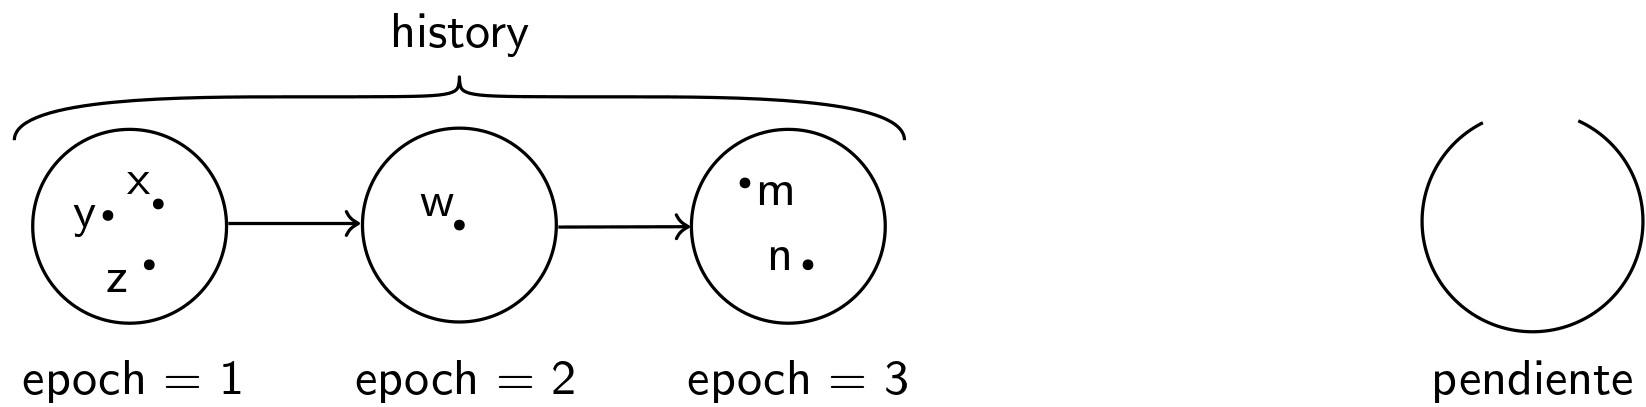
\includegraphics[width = 5in]{figures/setchain_api_02.png}\label{subfig:setchain-api-0}}\\
  \bigskip
  \subfloat[Un cliente invoca $v$.\<add>(a)]{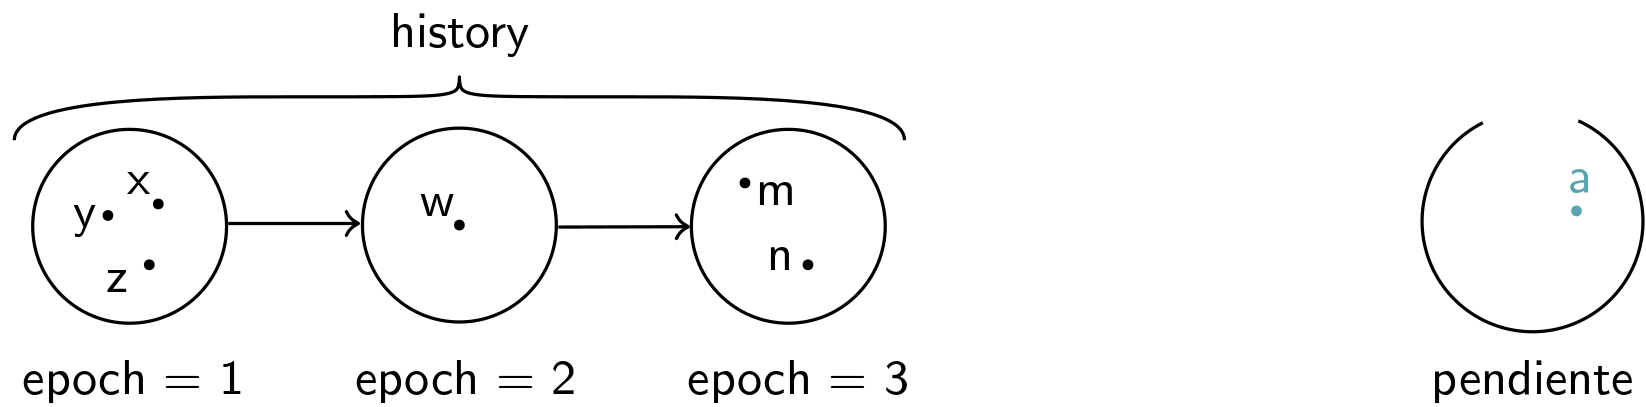
\includegraphics[width = 5in]{figures/setchain_api_12.png}\label{subfig:setchain-api-1}}\\
  \bigskip
  \subfloat[Un cliente invoca $v$.\<add>(b)]{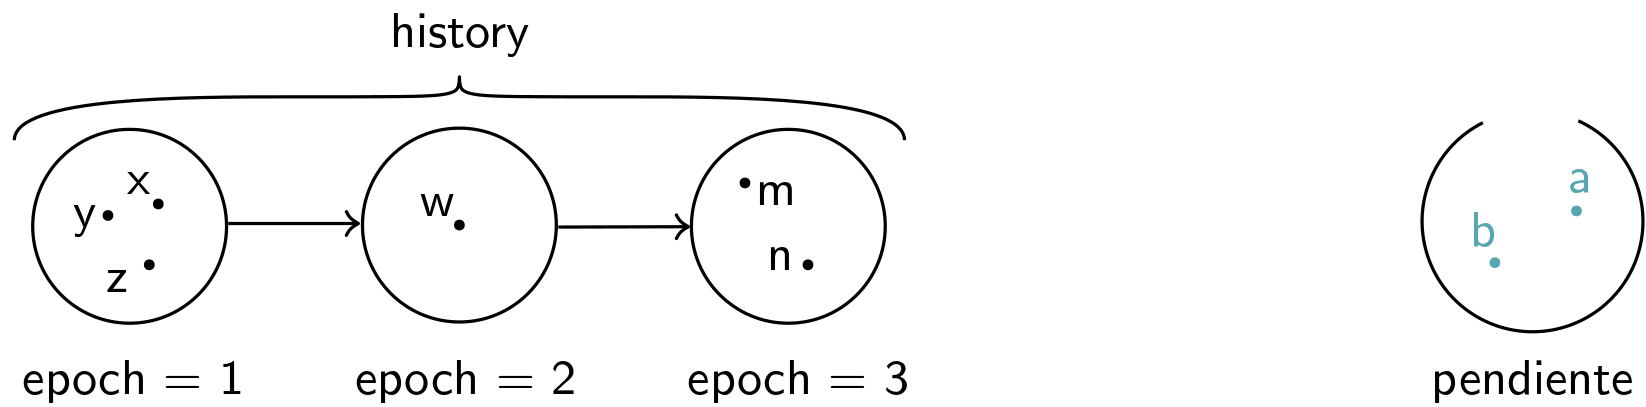
\includegraphics[width = 5in]{figures/setchain_api_23.png}\label{subfig:setchain-api-2}}\\
  \bigskip
  \subfloat[Ocurre un nuevo incremento de época]{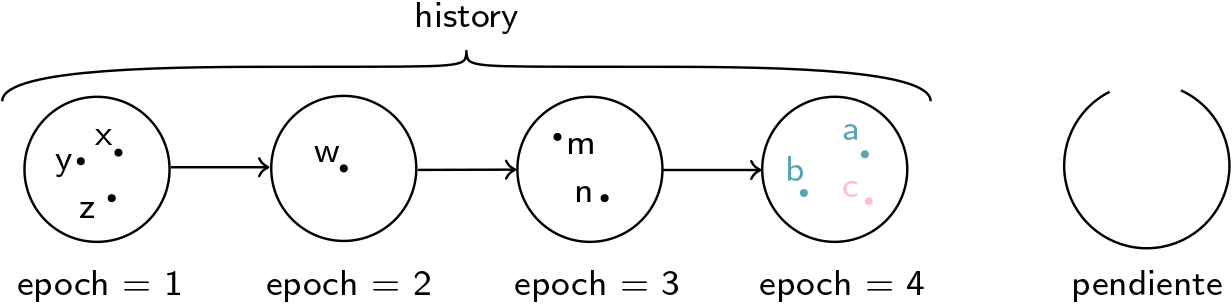
\includegraphics[width = 5in]{figures/setchain_api_33.png}\label{subfig:setchain-api-3}}
  \caption{Ejemplo de evolución de la \setchain}
  \label{fig:setchain-api-flow}
\end{figure}

En la Figura ~\ref{fig:setchain-api-flow} se muestra un breve ejemplo del funcionamiento de la \setchain.
%
Sea $v$ un servidor correcto que mantiene la \setchain.
%
En la Figura ~\ref{subfig:setchain-api-0} se muestra un estado posible para la \setchain desde el punto de vista
de $v$.
%
En dicho estado, la invocación $v$.\<get> por parte de un cliente resulta en la terna $(v.\THESET, v.\HISTORY, v.\EPOCH)$,
donde:
%donde $v.\THESET = \{x, y, z, w, m, n\}, \ v.\HISTORY = \{1: \{x, y, z\}, 2: \{w\}, 3: \{m, n\}\}, \ v.\EPOCH = 3$
%\[ (v.\THESET, v.\HISTORY, v.\EPOCH) \]
%donde
\[ v.\THESET = \{x, y, z, w, m, n\},\]
\[\ v.\HISTORY = \{1: \{x, y, z\}, 2: \{w\}, 3: \{m, n\}\},\]
\[\ v.\EPOCH = 3. \]


En la Figura ~\ref{subfig:setchain-api-1} y la Figura ~\ref{subfig:setchain-api-1} se presentan los resultados de un cliente
invocando $v$.\<add>(a) y $v$.\<add>(b), respectivamente.
%
Luego de añadir ambos elementos, se tiene:
\[ v.\<get> = (\{x, y, z, w, m, n, a, b\}, \{1: \{x, y, z\}, 2: \{w\}, 3: \{m, n\}\}, 3). \]
%
Es decir, el único cambio se percibe en el valor de $v.\THESET$ (que ahora incluye a los elementos $a$ y $b$).

Finalmente, en la Figura ~\ref{subfig:setchain-api-3} se muestra el estado de la \setchain luego de ejecutarse un nuevo
incremento de época.
%
Este evento tiene como consecuencia la creación de una nueva época que incluye a los elementos hasta entonces pendientes 
de ser estampados, en este caso $a$, $b$ y $c$.
%
Si bien el elemento $c$ no era conocido por el servidor $v$ previamente, los nodos servidores deciden colaborativamente
los nuevos elementos que son estampados.
%
En este sentido, se puede suponer que un cliente invocó $w.\<add>(c)$ sobre un servidor correcto $w$ y, por lo tanto,
$c$ pertenecía a $w.\THESET$.
%
De este modo, se tiene el nuevo punto de vista del servidor $v$:
\[ v.\<get> = (\{x, y, z, w, m, n, a, b, c\}, \{1: \{x, y, z\}, 2: \{w\}, 3: \{m, n\}, 4: \{a, b, c\}\}, 4). \]



\section{Propiedades}\label{subsubsec:setchain-properties}
Para asegurar correctitud, las implementaciones de \setchain deben satisfacer ciertas propiedades que
proveen garantías eventuales para elementos añadidos y garantía de consistencia entre los servidores
correctos.
%
Estas propiedades razonan sobre los servidores correctos, dado que los servidores bizantinos no proveen
ninguna garantía.

La primera propiedad establece que las épocas solo contienen elementos que provienen del conjunto
de solo crecimiento.
%
\newcounter{prop:consistent-set}
\setcounter{prop:consistent-set}{\value{property}}

\begin{property}[Consistent Sets]\label{api:consistent-set}
  Sea $(S,H,h)=v.\<get>()$ el resultado de una invocación a un servidor correcto $v$.
  %
  Luego, para cada $i\leq h, H(i) \subseteq S$.
\end{property}
%
La segunda propiedad declara que todo elemento añadido a un servidor correcto $v$ es eventualmente
retornado en todas las llamadas futuras a $v$.\<get>.
%
\begin{property}[Add-Get-Local]\label{api:history->theset-local}
  %Sea $e$ un elemento válido y $v.\<add>(e)$ una operación invocada en un servidor correcto $v$.
  Sea $e \in V$ y $v.\<add>(e)$ una operación invocada en un servidor correcto $v$.
  %
  Luego, eventualmente todas las invocaciones $(S,H,h)=v.\<get>()$ 
  satisfacen $e\in S$.
\end{property}
La siguiente propiedad establece que los elementos presentes en un servidor correcto son propagados
a todos los servidores correctos.

\begin{property}[Get-Global]\label{api:history->theset}
  Sean $v$ y $w$ dos servidores correctos,
  ${(S,H,h)=v.\<get>()}$ y $e \in U$.
  %
  Si $e \in S$, luego eventualmente todas las invocaciones
  $(S',H',h')=w.\<get>()$ satisfacen que $e \in S'$.
\end{property}
%

Como ya se mencionó anteriormente, a lo largo de este trabajo se asume que en cualquier momento
existe un instante futuro en el cual ocurre el próximo incremento de época.
Esta suposición es razonable ya que puede ser garantizada usando \textit{timeouts} en cualquier escenario práctico.
Luego, la siguiente propiedad establece que todos los elementos añadidos son eventualmente estampados
con un número de época.
%
\begin{property}[Eventual-Get]\label{api:theset->history}
  Sea $v$ un servidor correcto, $(S,H,h)=v.\<get>()$ y $e \in U$.
  % 
  Si $e \in S$, luego eventualmente todas las invocaciones
  $(S',H',h')=v.\<get>()$ satisfacen que $e \in H'$.
\end{property}

% % No sé si vale la pena poner una propiedad que se infiere de las anteriores
% Las tres propiedaes previas implican la siguiente propiedad.
% %
% \begin{property}[Get-After-Add]\label{api:get-after-add}
%   Sea $v.\<add>(e)$ una operación invocada en un servidor correcto $v$ con $e \in U$.
%   %
%   Luego, eventualmente todas las invocaciones $(S,H,h)=w.\<get>()$ en servidores correctos
%   $w$ satisfaccen que $e\in H$.
% \end{property}
% %

La siguiente propiedad establece que un elemento puede estar en a lo sumo una época.

%
\begin{property}[Unique Epoch]\label{api:local_unique_stamp}
  Sea $v$ un servidor correcto,
  $(S,H,h)=v.\<get>()$, e
  ${i,i'\leq{}h}$ con ${i\neq i'}$.
  %
  Luego, $H(i)\cap{}H(i')=\emptyset$.
\end{property}
%

La siguiente propiedad establece que los servidores están de acuerdo en el contenido
de las épocas.
%
\begin{property}[Consistent Gets]\label{api:consistent-gets}
  Sean $v$ y $w$ servidores correctos, $(S,H,h)=v.\<get>()$ y
  $(S',H',h')=w.\<get>()$, y sea $i\leq \min(h,h')$. Luego
  $H(i)=H'(i)$.
\end{property}

De las dos propiedades anteriores se deriva que ningún elemento puede estar en dos
épocas diferentes, incluso si los conjuntos que definen las épocas se
obtienen de invocaciones \<get> a distintos servidores (ambos correctos).


% Property~\ref{api:consistent-gets} states that the histories returned
% by two $\<get>$ invocations to correct servers are one the prefix of
% the other.
% %
% However, since two elements $e$ and $e'$ can be inserted at two
% different correct servers---which can take time to propagate---, the
% $\<theset>$ part of $\<get>$ obtained from two correct servers may not
% be contained in one another.

Finalmente, se requiere que todo elemento en $\THESET$ provenga del resultado de un cliente
añadiendo un elemento.

%
\begin{property}[Add-before-Get]\label{api:get->add}
  Sea $v$ un servidor correcto, $(S,H,h)=v.\<get>()$
  y $e \in S$.
  %
  Luego, hubo una operación $w.\<add>(e)$ en el pasado en algún servidor $w$.
\end{property}

Las propiedades~\ref{api:consistent-set}, \ref{api:local_unique_stamp},
\ref{api:consistent-gets} y \ref{api:get->add} son propiedades de \textit{safety}.
%
Las propiedades~\ref{api:history->theset-local}, \ref{api:history->theset},
y \ref{api:theset->history}
%\ref{api:get-after-add}
son propiedades de \textit{liveness}.

% \begin{itemize}
%   \item Cada elemento válido agregado en un servidor correcto eventualmente es retornado en
%   todas las futuras invocaciones a \<get> hechas sobre servidores correctos.
%   \item Todos los elementos válidos agregados en un servidor correcto deben eventualmente ser
%   estampados con un número de época en todos los servidores correctos.
%   \item Una vez que un elemento es estampado con una época, no puede ser des-estampado, ni puede
%   ser estampado con otro número de época.
%   \item Dos servidores correctos cualesquieras están de acuerdo en el contenido de todas las épocas
%   que hayan sido computadas~\footnote{No todos los servidores correctos procesan los incrementos de
%   época simultáneamente, dado que algunos pueden estar más atrasados que otros.}.
%   \item Cada elemento que se estampa con una época proviene del resultado de un cliente añadiendo
%   el elemento.
% \end{itemize}
% \gabina{Epoch proofs are part of the epoch but are not coming directly from the result of a client adding element.}
